\chapter{Memory}

\section{RAM access time}
In this part, Report latency for individual integer accesses to main memory and the L1 and L2 caches.

\paragraph{Methodology}
To test memory access latency, I first followed the procedure described in the lmbench paper, testing different stride lengths over varying sizes of arrays. But it is something like sequential access, I wrote code and got the test data, found that it is hard to distinguish different level cache.

Then I choose random access as my methodology. For different array size, I iterate 1 million times, each is random access.

The overhead of random generator and iterations are about  27 cycles.

\paragraph{Predictions}
Different level caches and main memory have different access cycles.

For L1-cache, we predict hardware cycles are 5 and software 2;
For L2-cache, we predict hardware cycles are 10 and software 4;
For L3-cache, we predict hardware cycles are 15 and software 6;
For main memory, we predict hardware cycles are 30 and software 10;

\paragraph{Results}
We present our measure results.

\begin{center}
\begin{tabular}{l*{6}{c}r}
Array size              & Hardware  & Software  & Overall  & Measured  & Remove Overhead \\
\hline
1KB & 5 & 2 & 7 & 28.116605 & 1.116605 \\
2KB & 5 & 2 & 7 & 28.864342 &  1.864342 \\
4KB & 5 & 2 & 7 & 27.687838  & 0.687838\\
8KB & 5 & 2 & 7 & 28.736381  & 1.736381\\
16KB & 5 & 2 & 7 & 28.449469  & 1.449469 \\
32KB & 6 & 3 & 9 & 28.104032  & 1.104032 \\
64KB & 12 & 4 & 16 & 27.939144 &  0.939144\\
128KB & 12 & 4 & 16 & 27.683588 &  0.683588\\
256KB & 14 & 4 & 18 & 28.151352 &  1.151352\\
512KB & 16 & 6 & 22 & 29.170154  & 2.170154 \\
1MB & 16 & 6 & 22 & 32.495250  & 5.495250\\
2MB & 16 & 6 & 22 & 35.461017 & 8.461017 \\
4MB & 20 & 8 & 28 & 47.772894  & 20.772894\\
8MB & 30 & 8 & 38 & 68.281862  & 41.281862\\
16MB & 40 & 10 & 50 & 78.474217 & 51.474217 \\
32MB & 40 & 10 & 50 & 86.430870 & 59.474217 \\
64MB & 40 & 10 & 50 & 84.635278 & 57.635278 \\
\end{tabular}
\end{center}

\begin{figure}[htbp] %  figure placement: here, top, bottom, or page
   \centering
   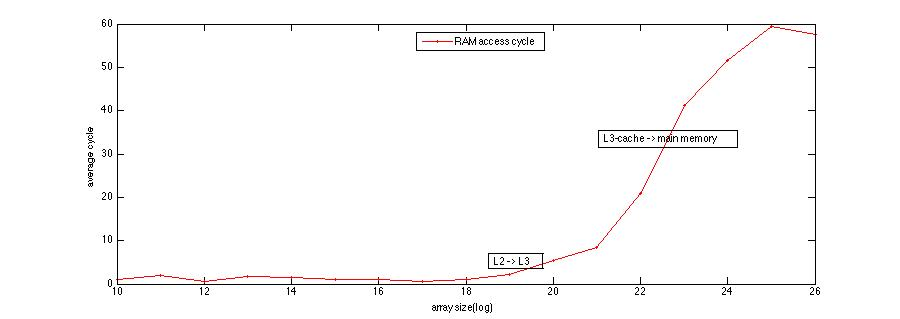
\includegraphics[width=6in]{./pics/ramacc.jpg} 
   \caption{RAM access}
   \label{fig:RAM access}
\end{figure}

\paragraph{Discussion}
It is easy to see the transition from L3-cache to main memory, it is very steep in the picture from array size 22 to 24. Because my L3-cache is 6MB, so it is between 22 and 24.

We can also see the transitions from L2-cache to L3-cache. In the picture, from 18 to 20, the access time increase. Because my L2-cache is 256KB, which is equal to 18 in the picture.

But I can't see the transition from L1-cache to L2-cache in the picture.

We can also see that within cache, the RAM access time cycles are very small compared to that of main memory access.